% sample: clutter rate=50, no. 096

We begin by examining the simplest scenario where the number of targets is constant in time and there are only two targets present in the scene. As mentioned before, we generated $100$ Monte Carlo measurement and clutter samples for every test scenario and parameter setting, given that the true trajectories of these objects do not change in time. Figure \ref{fig:c1-results-overview} shows one of these samples for the default filter settings described in Section \ref{sec:test-scenarios}. The left image displays how the true tracks of two objects are generated. The transition from black to yellow color illustrates the change in time for a target. The red stars represent the measurements that the filter receives at a time step, with the intensity of the red color representing the time step. Gray crosses indicate clutter measurements, with the intensity of the gray color having the same meaning as for the red stars. On the right side of the figure, we see the change of both coordinates in time with noise measurements and the estimates of the filter represented by black circles at each time step.

\begin{figure*}
    \centering
    \begin{subfigure}[]{0.48\linewidth}
        \centering
        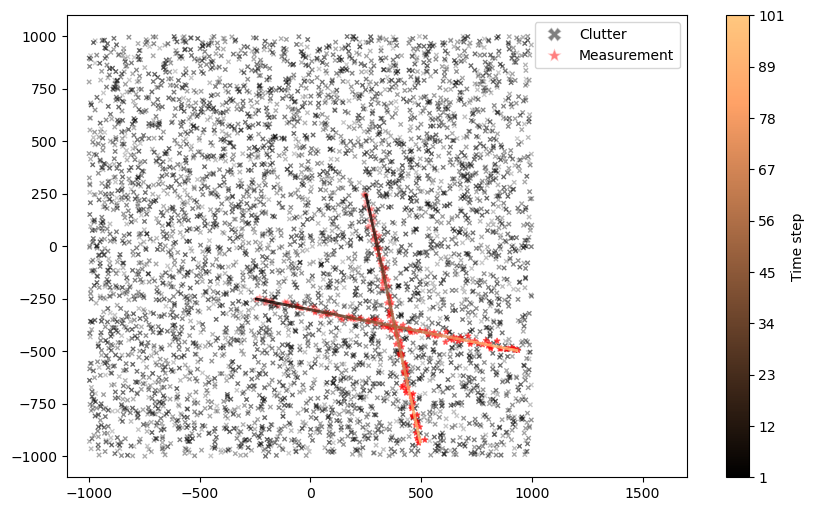
\includegraphics[width=\linewidth]{figures/c1-tracks-measurements.png}
    \end{subfigure}
    \hfill
    \begin{subfigure}[]{0.48\linewidth}
        \centering
        \begin{subfigure}[t]{\linewidth}
            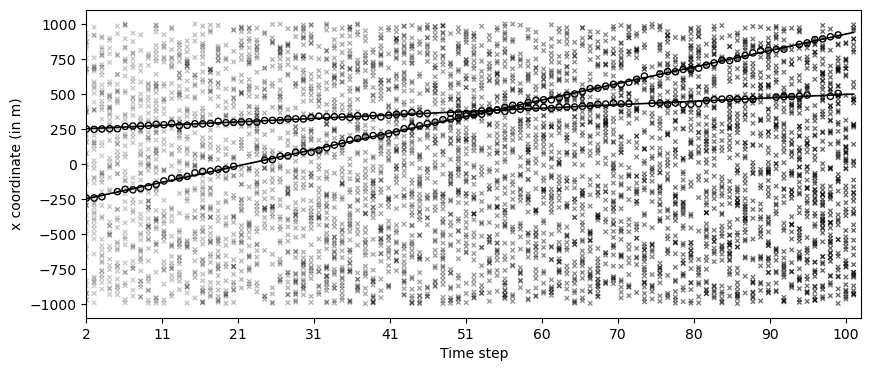
\includegraphics[width=\linewidth]{figures/c1-x-estimates.png}
        \end{subfigure}
        \vfill\par
        \begin{subfigure}[b]{\linewidth}
            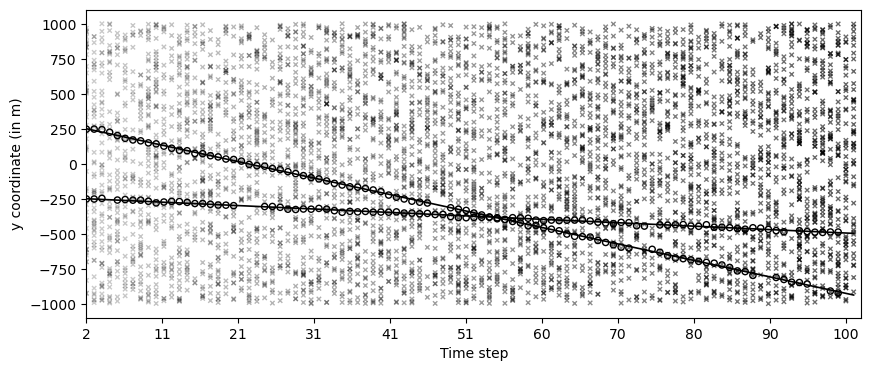
\includegraphics[width=\linewidth]{figures/c1-y-estimates.png}
        \end{subfigure}
    \end{subfigure}
  \caption[One sample of data and estimates for the (C1) scenario.]{One sample of data and estimates for the (C1) scenario. Left: True tracks of two objects (black to yellow) with clutter measurements (gray crosses) and received measurements (red stars) for a single Monte Carlo sample. Right: Change of both coordinates in time with noise measurements (red circles) and filter estimates (black circles) for the same Monte Carlo sample. The filter shows accurate estimates even in very cluttered environments.}
  \label{fig:c1-results-overview}
\end{figure*}

We can observe that the filter provides very accurate estimates even in cluttered environments. For instance, in this case, the filter receives an average of $50$ noise measurements for every measurement set. However, we also notice that estimates are not perfect. For instance, one of the objects did not receive estimates at time $k=21$ and it lasted for three time steps, and at $k=24$, the object appeared again.

Let us examine how changes in settings affect the filter performance in terms of metrics. To illustrate all runs for every parameter, we use a box plot. For every value of a parameter, we draw a box whose boundaries represent the first and third quartiles. The ``whiskers'' depict the minimum and maximum values of the distribution of metric values from all runs, and black dots represent those measurements that are considered outliers. The minimum and maximum values are calculated as one and a half times the interquartile range from the first and third quartiles, respectively, where the interquartile range is the difference between the two quartiles. Outliers are defined as those values that fall outside the range between the minimum and maximum. The black line inside boxes represents the median value, and the red dot is for the mean value. Means are connected to better see the overall trend. 

First, we examine the change of performance for different clutter rates. In Figure \ref{fig:c1-clutter}, we see that the increase of clutter measurements worsens the performance in both the precision of target estimates, and the estimate of the number of targets. It should be noted, that the increase in the expected absolute error is more pronounced than for the CPEP. It is clear that higher clutter rates causes more spurious estimates that the filter may consider to be real targets. Even in cases where these false tracks are not confirmed later, the number of estimated targets can be higher than the real number at a given time moment. However, in general, we see that the increase is not drastic, and the performance of the filter is good for even high values of the clutter rate.

\begin{figure}
    \centering
    \begin{subfigure}[]{0.48\linewidth}
        \centering
        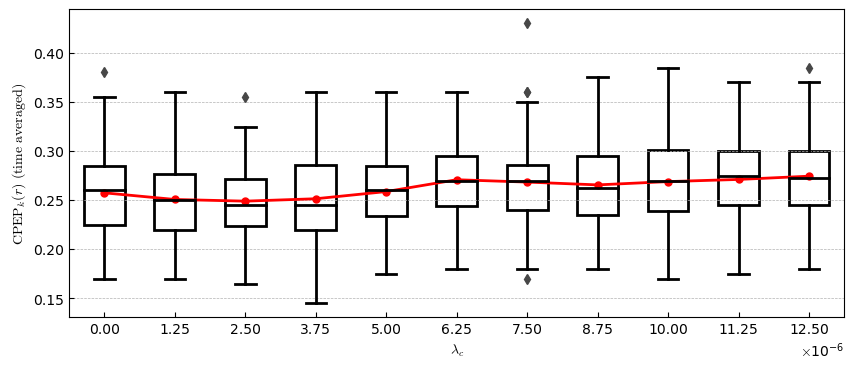
\includegraphics[width=\linewidth]{figures/c1-clutter-cpep.png}
    \end{subfigure}
    \hfill
    \begin{subfigure}[]{0.48\linewidth}
        \centering
        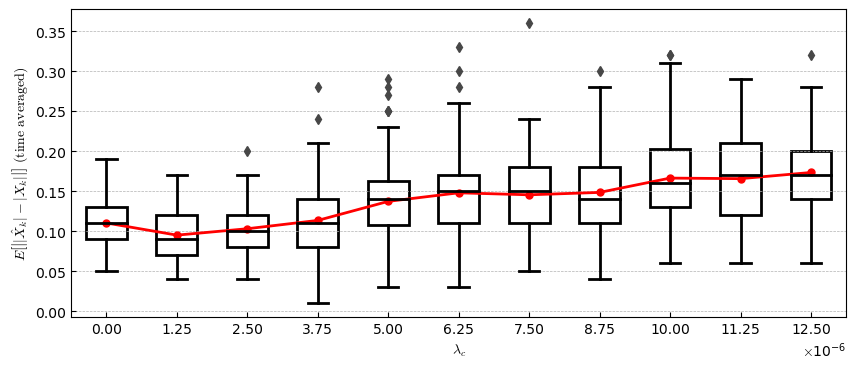
\includegraphics[width=\linewidth]{figures/c1-clutter-eae.png}
    \end{subfigure}
  \caption[(C1). Change of performance depending on the clutter rate.]{Here, we examine the change of CPEP (left) and the expected absolute error on the number of targets (right) for the (C1) scenario for different values of the clutter spatial rate $\lambda_c$. Every box is the representation of the distribution of $100$ independent samples. As the clutter spatial rate increases, the estimation error also increases, which may be observed on the growing trend of both metrics. All other setting are set to default values, i.e. $P_{D,k} = 0.98$, $P_{S,k} = 0.99$, $\tau = 10^{-5}$ and $U = 4$.}
  \label{fig:c1-clutter}
\end{figure}

Next, let us look how the filter behaves for different values of the detection probability. The detection probability is a parameter that may vary for different environments and sensors, and its setting may affect the overall tracking performance. Figure \ref{fig:c1-pd} shows how the estimation error changes for multiple settings of the detection probability. It can be seen that low detection probabilities influence the performance of the filter drastically in both the estimation of the number of targets and the precision of state estimates. For instance, the comparison of two values of $P_{D,k} = 0.7$ and $P_{D,k} = 1.0$ gives more than seven times better estimation results in terms of the number of targets and twice better results for the state estimation. This suggests that the GM-PHD filter may show poor results for higher clutter rates and lower detection probabilities.

\begin{figure}
    \centering
    \begin{subfigure}[]{0.48\linewidth}
        \centering
        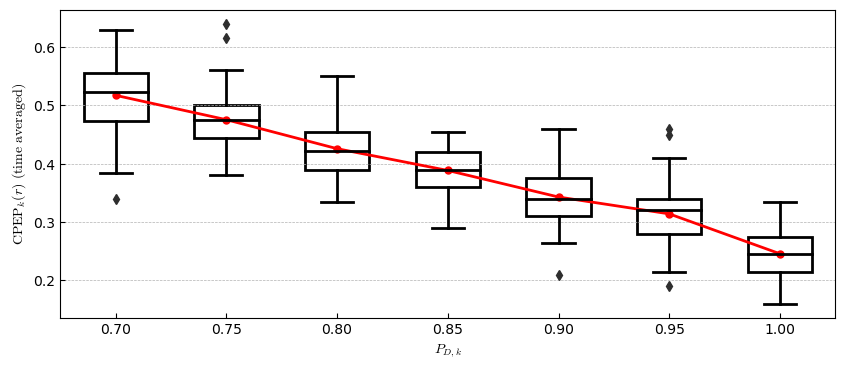
\includegraphics[width=\linewidth]{figures/c1-pd-cpep.png}
    \end{subfigure}
    \hfill
    \begin{subfigure}[]{0.48\linewidth}
        \centering
        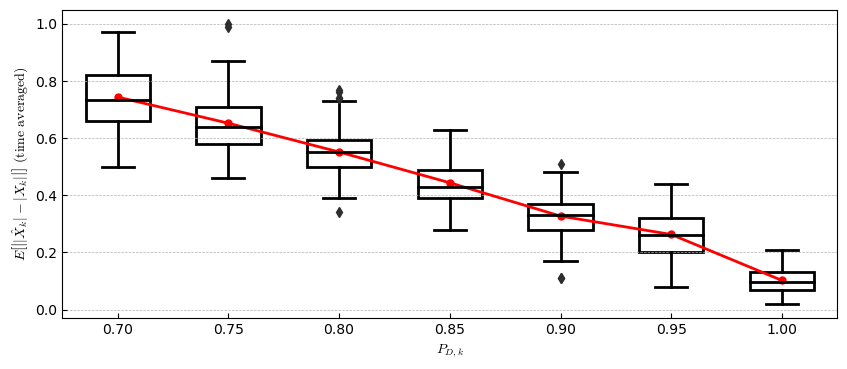
\includegraphics[width=\linewidth]{figures/c1-pd-eae.png}
    \end{subfigure}
  \caption[(C1). Change of performance depending on the detection probability.]{The change of CPEP (left) and the expected absolute error on the number of targets (right) for the (C1) scenario for different values of the detection probability $P_{D,k}$. Every box is the representation of the distribution of $100$ independent samples. As the detection probability increases, the estimation error decreases, which may be observed on the decreasing trend of both metrics. All other setting are set to default values, i.e. $\lambda_{c} = 12.5 \times 10^{-6}$, $P_{S,k} = 0.99$, $\tau = 10^{-5}$ and $U = 4$.}
  \label{fig:c1-pd}
\end{figure}

The third parameter we will examine is the probability of survival, $P_S$. In Figure \ref{fig:c1-ps}, we see that the performance is not affected by different values of the survival probability. The result suggests that even though the intensity of existing targets will rapidly decrease at every time step with a lower value of $P_{S,k}$, the tracks will still remain confirmed when the target generates enough measurements.

\begin{figure}
    \centering
    \begin{subfigure}[]{0.48\linewidth}
        \centering
        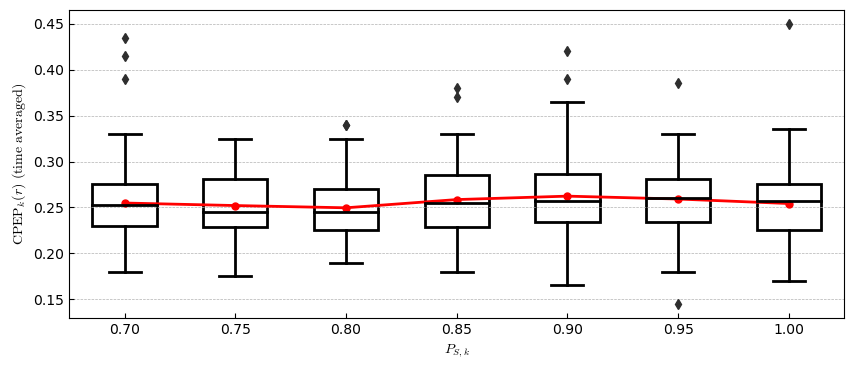
\includegraphics[width=\linewidth]{figures/c1-ps-cpep.png}
    \end{subfigure}
    \hfill
    \begin{subfigure}[]{0.48\linewidth}
        \centering
        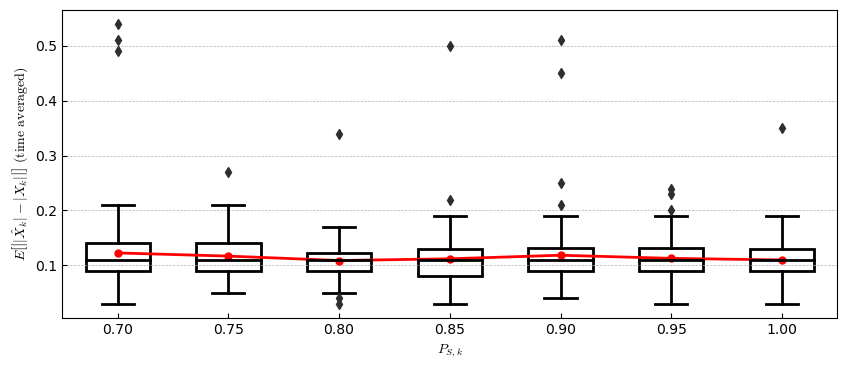
\includegraphics[width=\linewidth]{figures/c1-ps-eae.png}
    \end{subfigure}
  \caption[(C1). Change of performance depending on the survival probability.]{The change of CPEP (left) and the expected absolute error on the number of targets (right) for the (C1) scenario for different values of the survival probability $P_{S,k}$. Every box is the representation of the distribution of $100$ independent samples. Neither of metrics shows a change when the survival probability changes. All other setting are set to default values, i.e. $\lambda_{c} = 12.5 \times 10^{-6}$, $P_{D,k} = 0.98$, $\tau = 10^{-5}$ and $U = 4$.}
  \label{fig:c1-ps}
\end{figure}

The next variable parameter is the truncation threshold $\tau$. Figure \ref{fig:c1-tau} suggests that pruning too many components due to higher values of $\tau$ reduces the performance of the GM-PHD filter. For instance, $\tau = 10^{-3}$ caused a small decrease in both the precision and the estimate of the number of targets. The explanation of this effect is fairly straightforward. When the truncation threshold is too large, the number of hypotheses is drastically reduced at every time step and the loss of information in the posterior intensity is therefore not negligible.

\begin{figure}
    \centering
    \begin{subfigure}[]{0.48\linewidth}
        \centering
        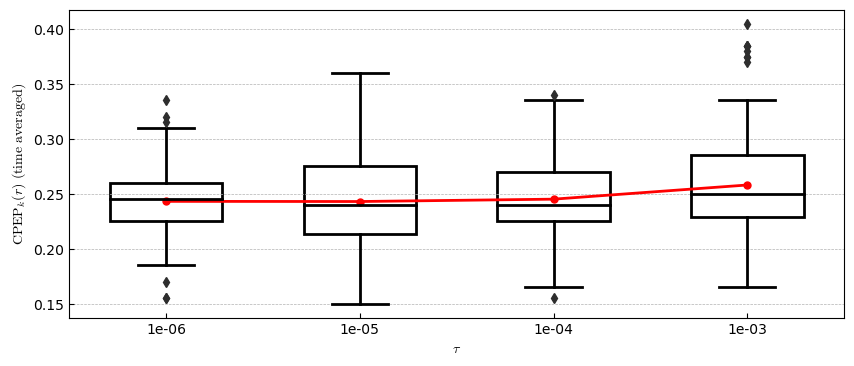
\includegraphics[width=\linewidth]{figures/c1-prune-cpep.png}
    \end{subfigure}
    \hfill
    \begin{subfigure}[]{0.48\linewidth}
        \centering
        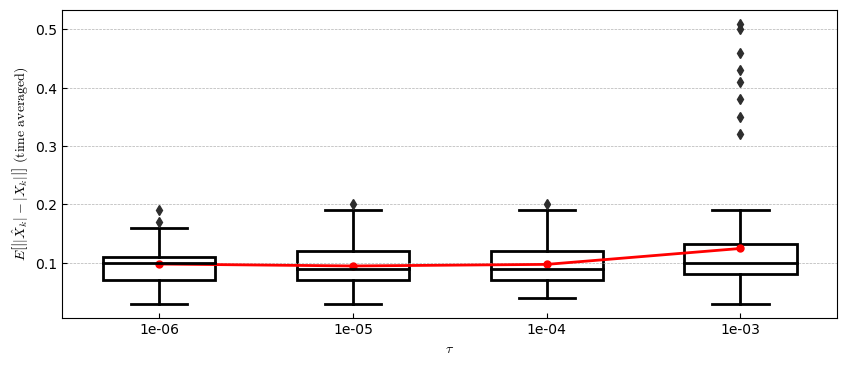
\includegraphics[width=\linewidth]{figures/c1-prune-eae.png}
    \end{subfigure}
  \caption[(C1). Change of performance depending on the prune threshold.]{The change of CPEP (left) and the expected absolute error on the number of targets (right) for the (C1) scenario for different values of the truncation threshold $\tau$. Every box is the representation of the distribution of $100$ independent samples. The X axis is on the logarithmic scale. We see, that, for higher values of $\tau$, the performance becomes worse. All other setting are set to default values, i.e. $\lambda_{c} = 12.5 \times 10^{-6}$, $P_{D,k} = 0.98$, $P_{S,k} = 0.99$ and $U = 4$.}
  \label{fig:c1-tau}
\end{figure}

The final parameter that was tested is the merge threshold $U$, or the maximum Mahalanobis distance between components on which these components will be merged into one. The results for different values of $U$ are shown in Figure \ref{fig:c1-u}. The increase in the distance between components causes the same effect as the increase of the truncation threshold $\tau$, that is, the loss of information from the posterior intensity. However, for this specific case and tested values of the parameter, the performance in both metrics worsens only slightly. The exact choice of the merge threshold $U$ is, however, domain-dependent.

\begin{figure}
    \centering
    \begin{subfigure}[]{0.48\linewidth}
        \centering
        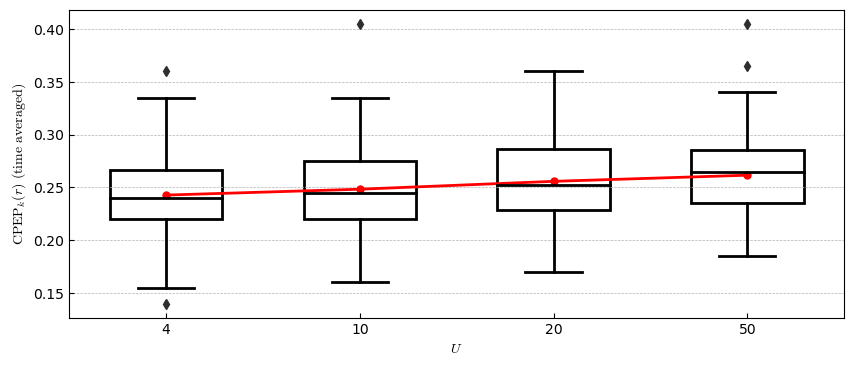
\includegraphics[width=\linewidth]{figures/c1-merge-cpep.png}
    \end{subfigure}
    \hfill
    \begin{subfigure}[]{0.48\linewidth}
        \centering
        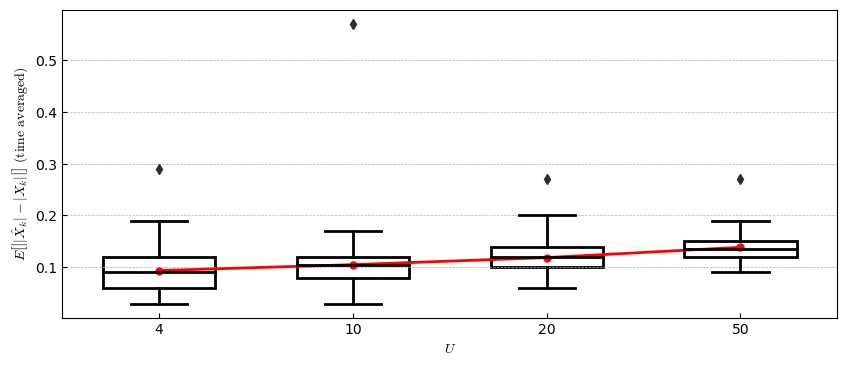
\includegraphics[width=\linewidth]{figures/c1-merge-eae.png}
    \end{subfigure}
  \caption[(C1). Change of performance depending on the merge threshold.]{The change of CPEP (left) and the expected absolute error on the number of targets (right) for the (C1) scenario for different values of the merge threshold $U$. Every box is the representation of the distribution of $100$ independent samples. The X axis does not have any scale. We see that, for higher values of $U$, the performance slightly worsens. All other settings are set to default values, i.e. $\lambda_{c} = 12.5 \times 10^{-6}$, $P_{D,k} = 0.98$, $P_{S,k} = 0.99$, and $\tau = 10^{-5}$.}
  \label{fig:c1-u}
\end{figure}

Finally, let us visually examine how trajectories are estimated and the final state of the posterior distribution. In Figure \ref{fig:c1-traj-post}, the left image illustrates the error in trajectory estimation. The track with the tag $667$ was terminated when two targets' paths cross each other, and the other track is created right after the intersection with a new tag $854$. We will later see how the effect of this problem worsens for more complex scenarios. However, we observe great results in terms of state estimation for both targets. The right image shows the internal state of the GM-PHD filter at time step $k=100$, more precisely the posterior intensity. It can be seen that two peaks are have expected value in the locations of two objects.

\begin{figure}
    \centering
    \begin{subfigure}[]{0.48\linewidth}
        \centering
        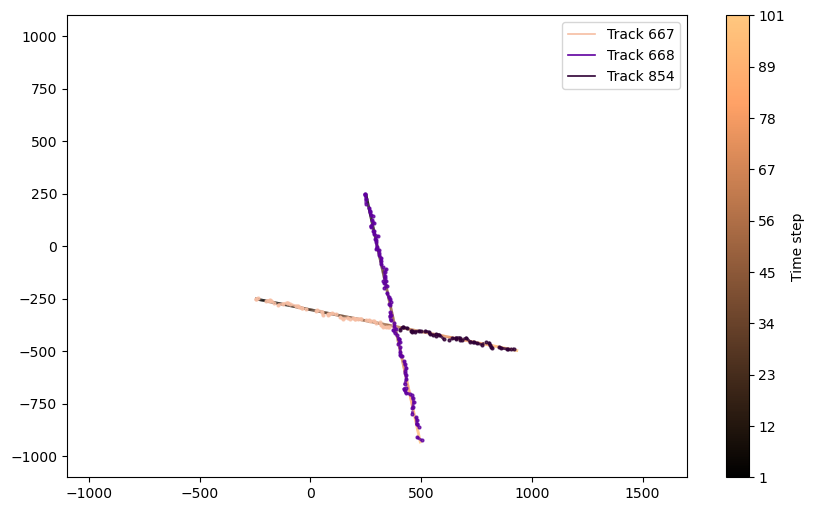
\includegraphics[width=\linewidth]{figures/c1-traj.png}
    \end{subfigure}
    \hfill
    \begin{subfigure}[]{0.48\linewidth}
        \centering
        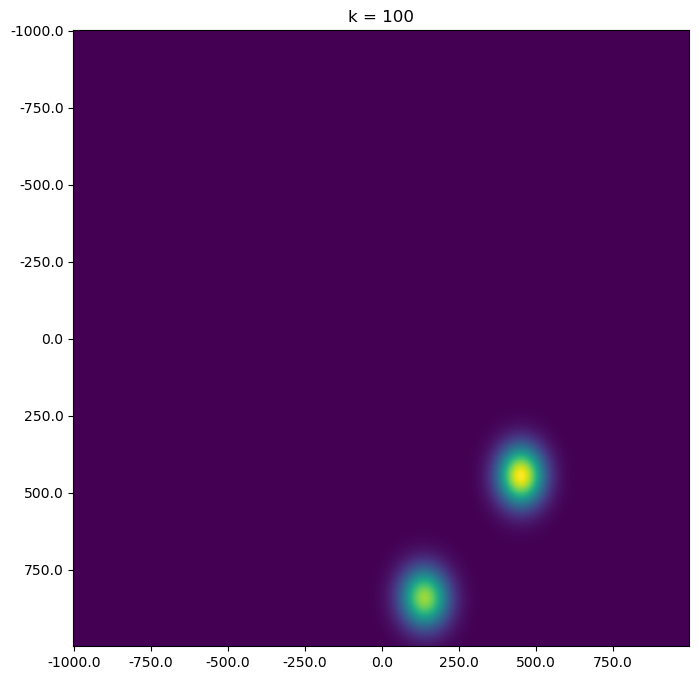
\includegraphics[width=\linewidth]{figures/c1-post.png}
    \end{subfigure}
  \caption[(C1). Trajectories estimations and the posterior intensity.]{Left: The visualization of trajectories estimates and the posterior distribution at time $k=100$. The straight gradient lines represent true tracks, the points represent state estimates generated by the GM-PHD filter, and different colors of the points illustrate unique tags of the estimated trajectories. Note, that when two tracks intersect, one of estimated tracks was falsely terminated and a new one created. Right: The posterior distribution at time step $k=100$. For visualization purposes, the covariance matrices of all Gaussian components were multiplied by the factor of $81$. Two Gaussian terms are visible on locations where two targets were at this time step. The bottom target has a lower weight, thus its color is dim. The filter was run with default settings, i.e. $\lambda_{c} = 12.5 \times 10^{-6}$, $P_{D,k} = 0.98$, $P_{S,k} = 0.99$, $\tau = 10^{-5}$, and $U=4$.}
  \label{fig:c1-traj-post}
\end{figure}
